\documentclass{report}
\usepackage[utf8]{inputenc}
%police et mise en page (marges) du document
\usepackage[T1]{fontenc}
\usepackage[top=3.6cm, bottom=2.4cm, left=3.2cm, right=3.2cm]{geometry}
\usepackage[frenchb]{babel}
\usepackage{hyperref}
\usepackage{graphicx}
\graphicspath{{images/}}
%Paragraph formatting
\setlength{\parindent}{0em}
\setlength{\parskip}{1em}
\renewcommand{\baselinestretch}{1.05}
%Personnalisation les en-têtes et pieds de page avec l'extension fancyhdr
\usepackage{fancyhdr}
\pagestyle{fancy}
\fancyfoot{}
\fancyhead[L]{\bfseries\thepage}
\fancyhead[R]{\bfseries\nouppercase{\leftmark}}
\setlength{\headheight}{15pt}

\let\headruleORIG\headrule
\renewcommand{\headrule}{\color{black} \headruleORIG}
\renewcommand{\headrulewidth}{1.0pt}
\usepackage{colortbl}
\arrayrulecolor{black}

\fancypagestyle{plain}{
  \fancyhead{}
  \fancyfoot[C]{\thepage}
  \renewcommand{\headrulewidth}{0pt}
}

\begin{document}
%%%%%%%%%%%%%%%%%%
%%% First page %%%
%%%%%%%%%%%%%%%%%%
\begin{titlepage}
\begin{center}


\includegraphics[width=0.6\textwidth]{logo_ecn}\\[1cm]

{\large Rapport de stage ingénieur}\\[0.5cm]

{\large STING}\\[0.5cm]

% Title
\rule{\linewidth}{0.5mm} \\[0.4cm]
{ \huge \bfseries Project DN-Rider en grails \\[0.4cm] }
\rule{\linewidth}{0.5mm} \\[1.5cm]

% Author and supervisor
\noindent
\begin{minipage}{0.4\textwidth}
  \begin{flushleft} \large
    \emph{Auteurs :}\\
    M. Guoxin \textsc{SUI}\\
  \end{flushleft}
\end{minipage}%
\begin{minipage}{0.4\textwidth}
  \begin{flushright} \large
    \emph{Encadrants :} \\
    M.~Jean-Michel \textsc{SIZUN}\\
    M.~Jérémy \textsc{RECHET}
  \end{flushright}
\end{minipage}

\vfill

% Bottom of the page
{\large \today}

\end{center}
\end{titlepage}


%%%%%%%%%%%%%%%%%%%%%%%%%%%%%
%%% Non-significant pages %%%
%%%%%%%%%%%%%%%%%%%%%%%%%%%%%

\chapter*{Remerciements}

\paragraph{} Je tiens d’abord à remercier l’entreprise VSCT et le service Efficacité opérationnelle de
m’avoir accueilli pour ces 20 semaines de stage et de m’avoir offert la possibilité de découvrir le
domaine de l'informatique' avec les sujets assez intéressants.
\paragraph{} Je souhaite particulièrement remercier mon tuteur de mon stage, Jean-Michel SIZUN, spécialiste projet
attaché au service Efficacité Opérationnelle, de m’avoir accordée ses conseils et ses soutiens qui
ont mené à bien une grande partie de mes missions de stage. J’ai eu l’opportunité de profiter de
son expérience pour l’avancement de mon projet et d'avoir un rôle d’ingénieur dans l’entreprise.
\paragraph{} Simultanément, je tiens aussi à remercier Jérémy RECHET, référent Process et fondamentaux
attachée à notre équipe et aussi la responsable du Pôle judiciaire. Elle m’a posé une bonne
fondation du projet et m’a prêté sa main en suivant le projet en même temps.
\paragraph{} Pour le projet Process Map, je remercie par ailleurs Aurore Dit Le Cadet, référent Process et
fondamentaux au service Efficacité Opérationnelle, pour sa disponibilité de me donner les
renseignements et m’accompagner lorsque nécessaire.
\paragraph{} Enfin, mes remerciements s’adressent également à l’ensemble du personnel de l’entreprise, en
particulier mes compagnons attachés à la même équipe avec moi pour leur soutien afin de
m’intégrer plus rapidement dans l’environnement de travail. Les gestionnaires qui étaient affectés
pour répondre à mes questions méritent également d’être tout particulièrement remerciées.

\tableofcontents

\chapter{Introduction}
\label{chap:Introduction}

Dans le cadre de ma deuxième année à l'Ecole Centrale de Nantes en suivant l'option informatique,
j'ai eu la chance d'effectuer un stage d'ingénieur de 20 semaines au sein de VSC Technologies.

En accompagnant de mon tuteur et d'un référent technique, j'ai développé une application web pour le projet "DN-Rider".

Le développement est organisé en méthode agiles, on essaie de pratiquer les principes de SCRUM.

L'applcation contient des parties IHM, API REST, documentation et intégration continue.
Un série de frameworks et langages ont été utilisés : Grails, Groovy, Bootstrap, jQuery, jQueryUI, HTML, CSS et JavaScript.

Ce rapport apporte le déroulement de ce stage, les connaissances et résultats obtenus au cours de mon stage.

\chapter{Contexte}

\section{SNCF \& VSC Technologies}
\subsection{Groupe SNCF}
La Société nationale des chemins de fer français (SNCF) est l'entreprise ferroviaire publique française, officiellement créée le 1er janvier 1938 en application du décret-loi du 31 août 1937. Elle est notamment présente dans les domaines du transport de voyageurs, du transport de marchandises et réalise la gestion, l'exploitation et la maintenance du réseau ferré national dont elle est propriétaire.

La SNCF est composée de trois EPIC (fig.\ref{fig:sncf_epic}), mais elle possède de nombreuses filiales aussi bien de droit public que de droit privé qui forment le groupe SNCF.

\begin{figure}[ht]
\centering
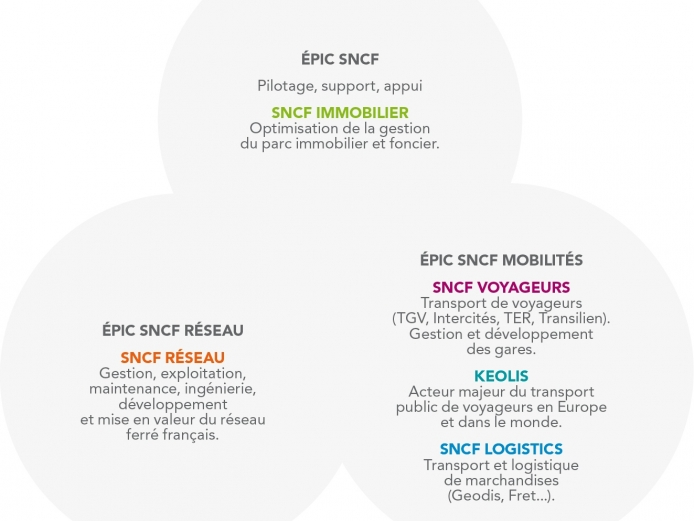
\includegraphics[width=0.8\textwidth]{sncf_epic}
\caption{Epic SNCF}
\label{fig:sncf_epic}
\end{figure}

Depuis le 1er janvier 2015, la SNCF est constituée de trois établissements publics à caractère industriel et commercial (EPIC) : l'EPIC de tête « SNCF » chargé du pilotage stratégique du groupe, « SNCF Réseau » propriétaire et gestionnaire du réseau ferré national et « SNCF Mobilités » chargé de l'exploitation des trains4,5.

La SNCF est donc une entreprise ferroviaire « intégrée » : elle exerce à la fois le métier d'exploitant (voyageurs et marchandises) et celui de gestionnaire d'infrastructure ferroviaire.

La Société nationale des chemins de fer français est devenue un établissement public à caractère industriel et commercial en 19836, alors qu'elle était auparavant une société anonyme d'économie mixte.

En 2015, le réseau ferré national propriété de SNCF Réseau compte environ 30 000 km de lignes dont 15 687 km de lignes électrifiées et 2 024 km de lignes à grande vitesse7. La même année, les effectifs des trois EPIC étaient de 149 500 salariés.

Chaque jour, elle fait circuler 15 000 trains de fret et de voyageurs et transporte plus de cinq millions de voyageurs8. Par son volume d'activité et la taille de son réseau, c'est la troisième entreprise ferroviaire européenne, après la Deutsche Bahn et les chemins de fer russes.

Elle détient des participations majoritaires ou totales dans des sociétés de droit privé regroupées dans le groupe SNCF et dont la tutelle de l'État est exercée par la Direction générale des infrastructures, des transports et de la mer du ministère de l'écologie, du développement durable et de l'énergie.9 Le siège social de la SNCF se trouve à La Plaine St-Denis, 2 place aux étoiles, à côté de la gare Stade de France Saint-Denis du RER D.

En 2014, la SNCF a enregistré un résultat net de 605 millions d'euros (contre une perte nette de 180 millions d'euros en 2013). L'EPIC SNCF Mobilités a réalisé un chiffre d'affaires de 27,2 milliards d'euros10.

Le reste du groupe SNCF, qui a réalisé 7,1 milliards d'euros de chiffre d'affaires en 200911, intervient dans les domaines suivants : logistique et transport routier de marchandises, transport routier de voyageurs (Keolis), liaison maritime (SeaFrance), ingénierie (EFFIA, INEXIA, commerce en ligne (Voyages-sncf.com), billettique (RITMx). Le groupe possède aussi des participations dans des sociétés ferroviaire et gestionnaires d'infrastructure portuaire partagées avec d'autres partenaires comme Eurostar, Thalys, Elipsos, Lyria et Nuovo Trasporto Viaggiatori.

\clearpage

\subsection{LE GROUPE VSC \& Rail Europe}
Le Groupe VSC et Rail Europe, filiale du Groupe SNCF, dirigée par Franck Gervais, est un acteur majeur du tourisme, expert de la distribution du train mais aussi de la vente des billets d'avions, de séjours, location de voitures et chambres d'hôtel, en France et en Europe. En 2015, son volume d’affaires atteint 4,1 milliards d’euros, en recul de 1,4\% par rapport à 2015 en vendant 86 millions de voyages, en croissance de 4,4\%. L’innovation demeure un axe central et exprime la capacité de Voyages-sncf.com à répondre aux nouveaux usages de ses clients. Aujourd’hui, en France, Voyages-sncf.com est le premier site d’e-commerce et la première agence de voyages en ligne ; le groupe rassemble 1200 collaborateurs dans le monde dont 40\% à l'international (130 en Europe et 350 hors Europe).

\begin{figure}[ht]
\centering

\includegraphics[width=0.9\textwidth]{vsct}
\caption{VSC Technologies: Un mix}
\label{fig:vsct}
\end{figure}

En 2000, le site internet Voyages-sncf.com est lancé sur le périmètre France. L’entreprise est à l’époque le distributeur unique des billets de train SNCF, et a pour objectif de transformer son site en portail de voyages offrant des produits et services complémentaires au train. L’année suivante, Voyages-sncf.com forme une joint-venture avec l’américain Expedia et devient une agence de voyage globale. L’entreprise poursuit alors son développement en France, tout en nourrissant une ambition internationale.

Pour répondre aux enjeux de la distribution du voyage et aux nouveaux comportements d’achats, le groupe VSC offre à ses clients mondiaux un réseau puissant, souple et adapté à leurs besoins. Il couvre plus présent dans 11 pays européens et 45 dans le reste du monde via un total de 67 sites internet et mobiles, 4 boutiques et un service de call-center. Afin de répondre aux enjeux spécifiques du marché B2B, le site Voyages-sncf.eu a été lancé en Europe en 12 langues (hors France).
Le site recense plusieurs transporteurs tels que SNCF, TER, Eurostar, Thalys, TGV Lyria ; 3 compagnies de bus, 400 compagnies aériennes ; 280 000 hôtels référencés ; plus de 25 000 offres de séjours ; 30 loueurs de voitures, etc.

Le groupe va bientôt se nomer "oui.sncf".
\clearpage

\section{Usine Logicielle \& Katana} (à quoi ça sert NDL)
\subsection{Usine Logicielle}
L'usine logicielle est l'ensemble de logiciels, d'outils et de procédures qui permettent de structurer et d'industrialiser les développements VSCT, ainsi que leur validation et déploiement sur l'infrastructure VSCT (hors VSCloud).

Dans sa définition actuelle: elle est la continuation de la Nouvelle usine logicielle Lille, et de Katana.

\begin{figure}[ht]
\centering
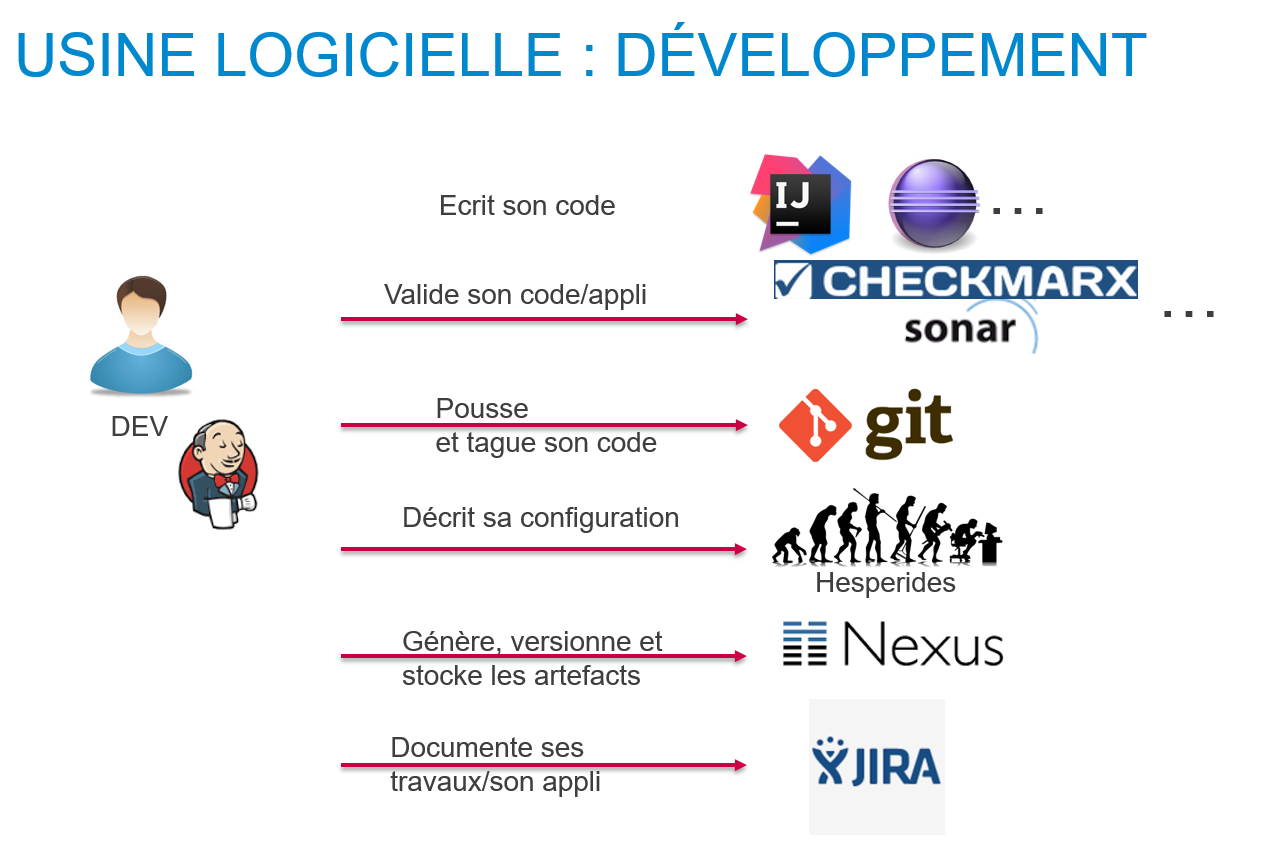
\includegraphics[width=0.8\textwidth]{usine-logicielle-developpement}
\caption{Usine Logicielle: Développement}
\end{figure}

Le développeur édite ses sources sur son poste de travail et les versionne sous GIT, avec entreposage dans une forge GITLAB .

L'application fait elle-même l'objet de versions formalisées, avec les livrables individuels packagés et archivés sur un entrepôt de binaires ( NEXUS ).

Pour chaque application, plusieurs plateformes sont montées sur l'infrastructure pour installer l'application.

Chaque plateforme a un rôle défini. Les plateformes de production font l'objet d'une gestion spécifique, le plus souvent pilotée par les équipes d'exploitation.

Le développeur dispose d'un outillage d'intégration/déploiement continue ( JENKINS ) pour piloter les compilations/générations, validations, déploiements sur des plateforme intermédiaires...
Pour certaines de ces étapes, JENKINS pilote des outils-tiers ( FISHEYE , CRUCIBLE , CHECKMARX , SONAR , ...).

Les serveurs (virtuels ou non) des plateformes sont accessibles en ligne de commande SSH au travers d'un frontal WALLIX, en fonction des droits de chacun.

Un frontal web ( RUNDECK ) permet de mettre à disposition des utilisateurs des opérations de plus haut-niveau, en self-service web sur les serveurs/plateformes (ex: déploiement applicatif, reconfiguration applicative, arrêt/relance et autres opérations spécifiques sur les serveurs).

\begin{figure}[ht]
\centering
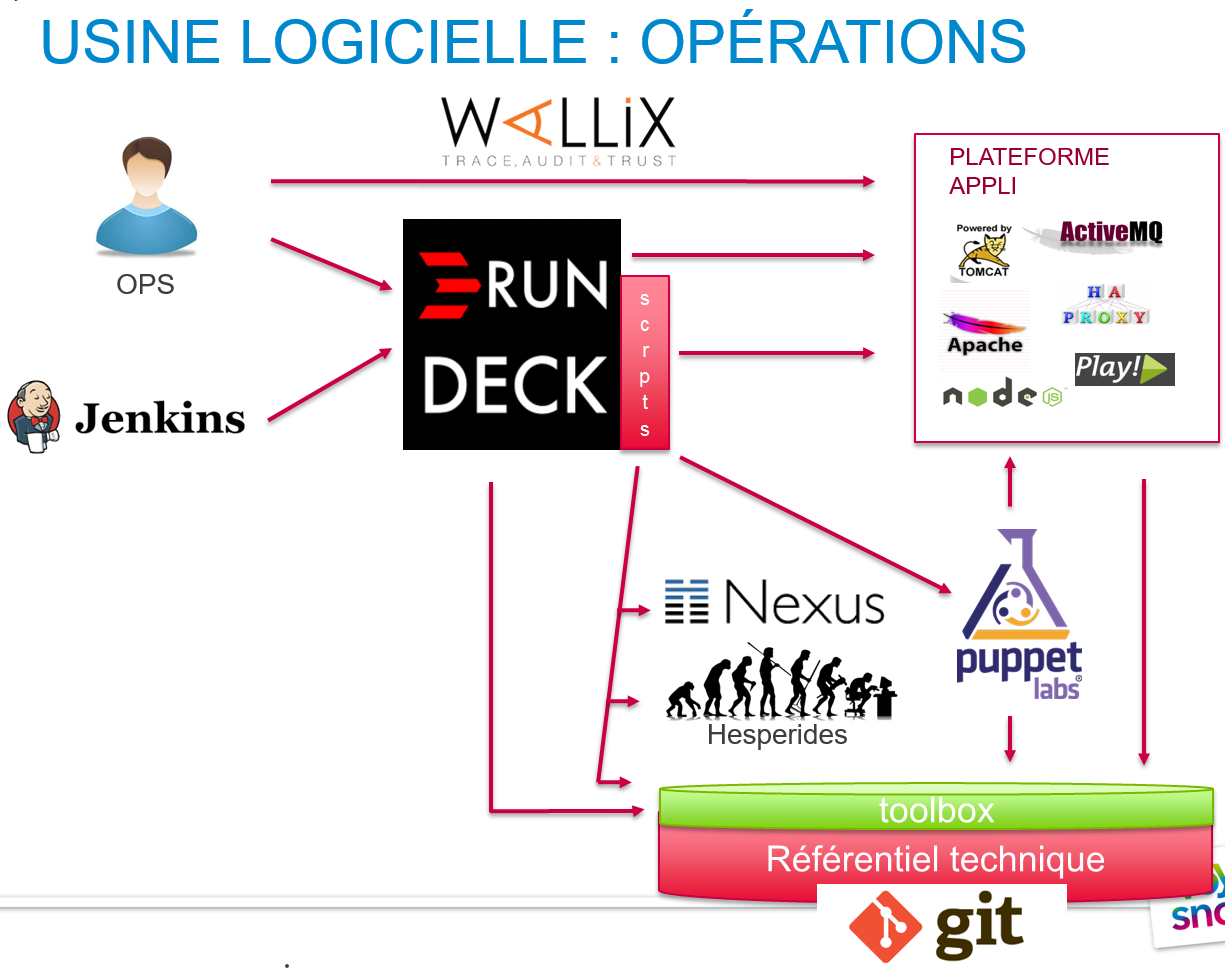
\includegraphics[width=0.8\textwidth]{usine-logicielle-operation}
\caption{Usine Logicielle: Opération}
\end{figure}

La configuration détaillée des différentes plateformes de l'application est industrialisée par:
\begin{itemize}
  \item l'outil PUPPET (configuration technique - COTS) et un REFERENTIEL TECHNIQUE en infra-as-code
  \item l'outil HESPERIDES (configuration application - développement VSCT en open-source)
\end{itemize}

Sauf cas particulier, l'accès aux outils et aux plateformes se fait selon l'authentification Active Directory de l'utilisateur.
\subsection{Katana}

La solution Katana assure la configuration technique, le déploiement applicatif et autre tâches industrialisées sur les machines des infrastructures VSC(T) de Lille/St-Denis (DMZs hors-production, Assemblage, Perf, Partenaires, Rithmics, Technique, Production, SNB....), à l'exception notable des SIs du CNIT, de VSCloud, et des infra bigData....

\begin{figure}[ht]
\centering
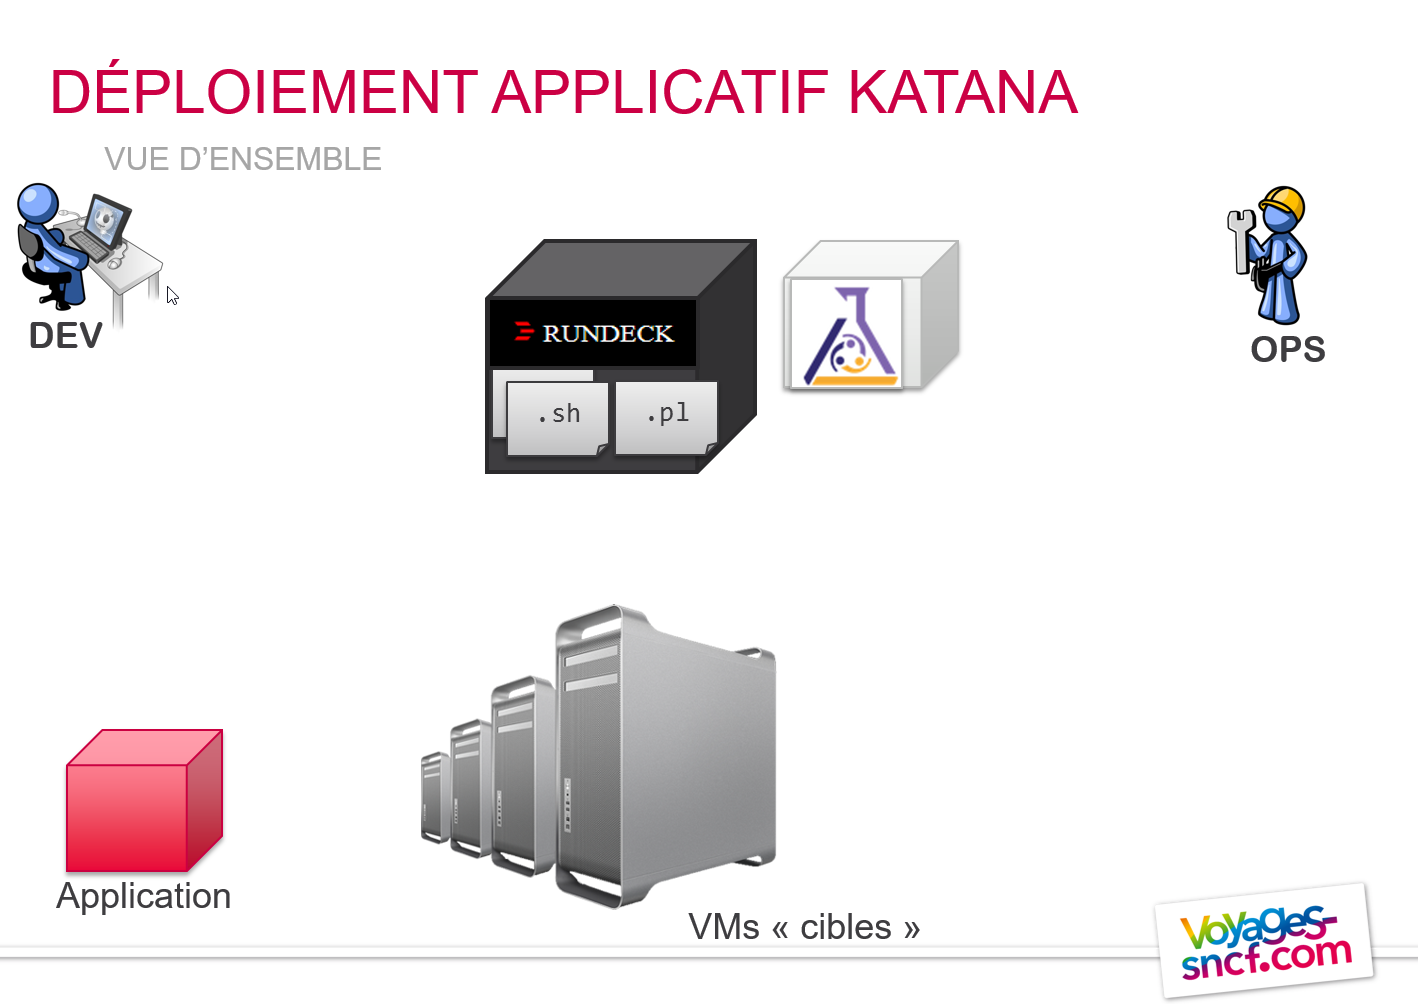
\includegraphics[width=0.8\textwidth]{katana}
\caption{Déploiement Applicatif Katana}
\end{figure}

Elle est composée de:

\begin{itemize}
  \item un référentiel de données techniques sur les plateformes/machines sous forme infraAsCode (fichiers envYyaml pour les plateformes, fichiers de configuration Puppet)
  \item un référentiel des configurations applicatives: Hesperides (géré par sa propre communauté)
  \item un catalogue de scripts (bash/perl/groovy/...), issu des projets de déploiement VSCT, implantant les opérations de déploiement/contrôle/supervision/etc
  \item un orchestrateur de tâches en self-service, Rundeck, qui pilote les tâches du Puppet et du catalogue de script (en central, ou sur les machines) .Il peut être contrôlé soit manuellement (par son IHM web), soit par API REST.
\end{itemize}

Katana s'inscrit dans la Usine Logicielle VSCT. La solution s'intègre en particulier avec les outils:
\begin{itemize}
  \item Jenkins: peut piloter l'orchestrateur de tâches dans le cadre des processus d'intégration ou de déploiement continus
  \item Nexus: pour le stockage des livrables applicatifs et autres artefacts (en particulier la (lexique. \ref{lexi:delivery_note}), le catalogue de scripts, les projets rundeck....)
  \item GIT: pour le stockage et le versionnement des fichiers (code du catalogue de scripts, référentiels de données enYaml, fichiers de configuration Puppet, ...)
\end{itemize}

\chapter{Projet DN-Rider}
\label{chap:Projet DN-Rider}

\section{Constat \& Objectif du stage}


Objectif: une application web (IHM + API REST) pour manipuler les notes de livraison Katana:

\begin{itemize}
  \item gérer l'objet NDL de manière plus simple qu'avec nexus/filesystème
  \item éviter les tableaux de suivi, type notes d'installation / tableaux de dépendances / ..., édités manuellement
  \item fédérer certaines fonctionnalités (extraction d'information, identification des package a installer sur une plateforme...) par rapport aux scripts bash/groovy/perl/ruby....
  \item  outiller le suivi du cycle de vie des versions par rapports aux infos remontées par les outils de l'usine logicielle et Katana
\end{itemize}

L’application devra être légère, dynamique et facilement évolutive, et non-contraignante pour les équipes.

Le but est de fiabiliser le processus de livraison/mise en production des applications.
\clearpage

\section{Contexte \& Démarche}
\paragraph{Equipe Intégration / Accompagnement Projet (transverse)}
\paragraph{Travail autonomie / equipe}
\paragraph{Démarche agile ( kanban) (devops)}

\begin{figure}[h]
\centering
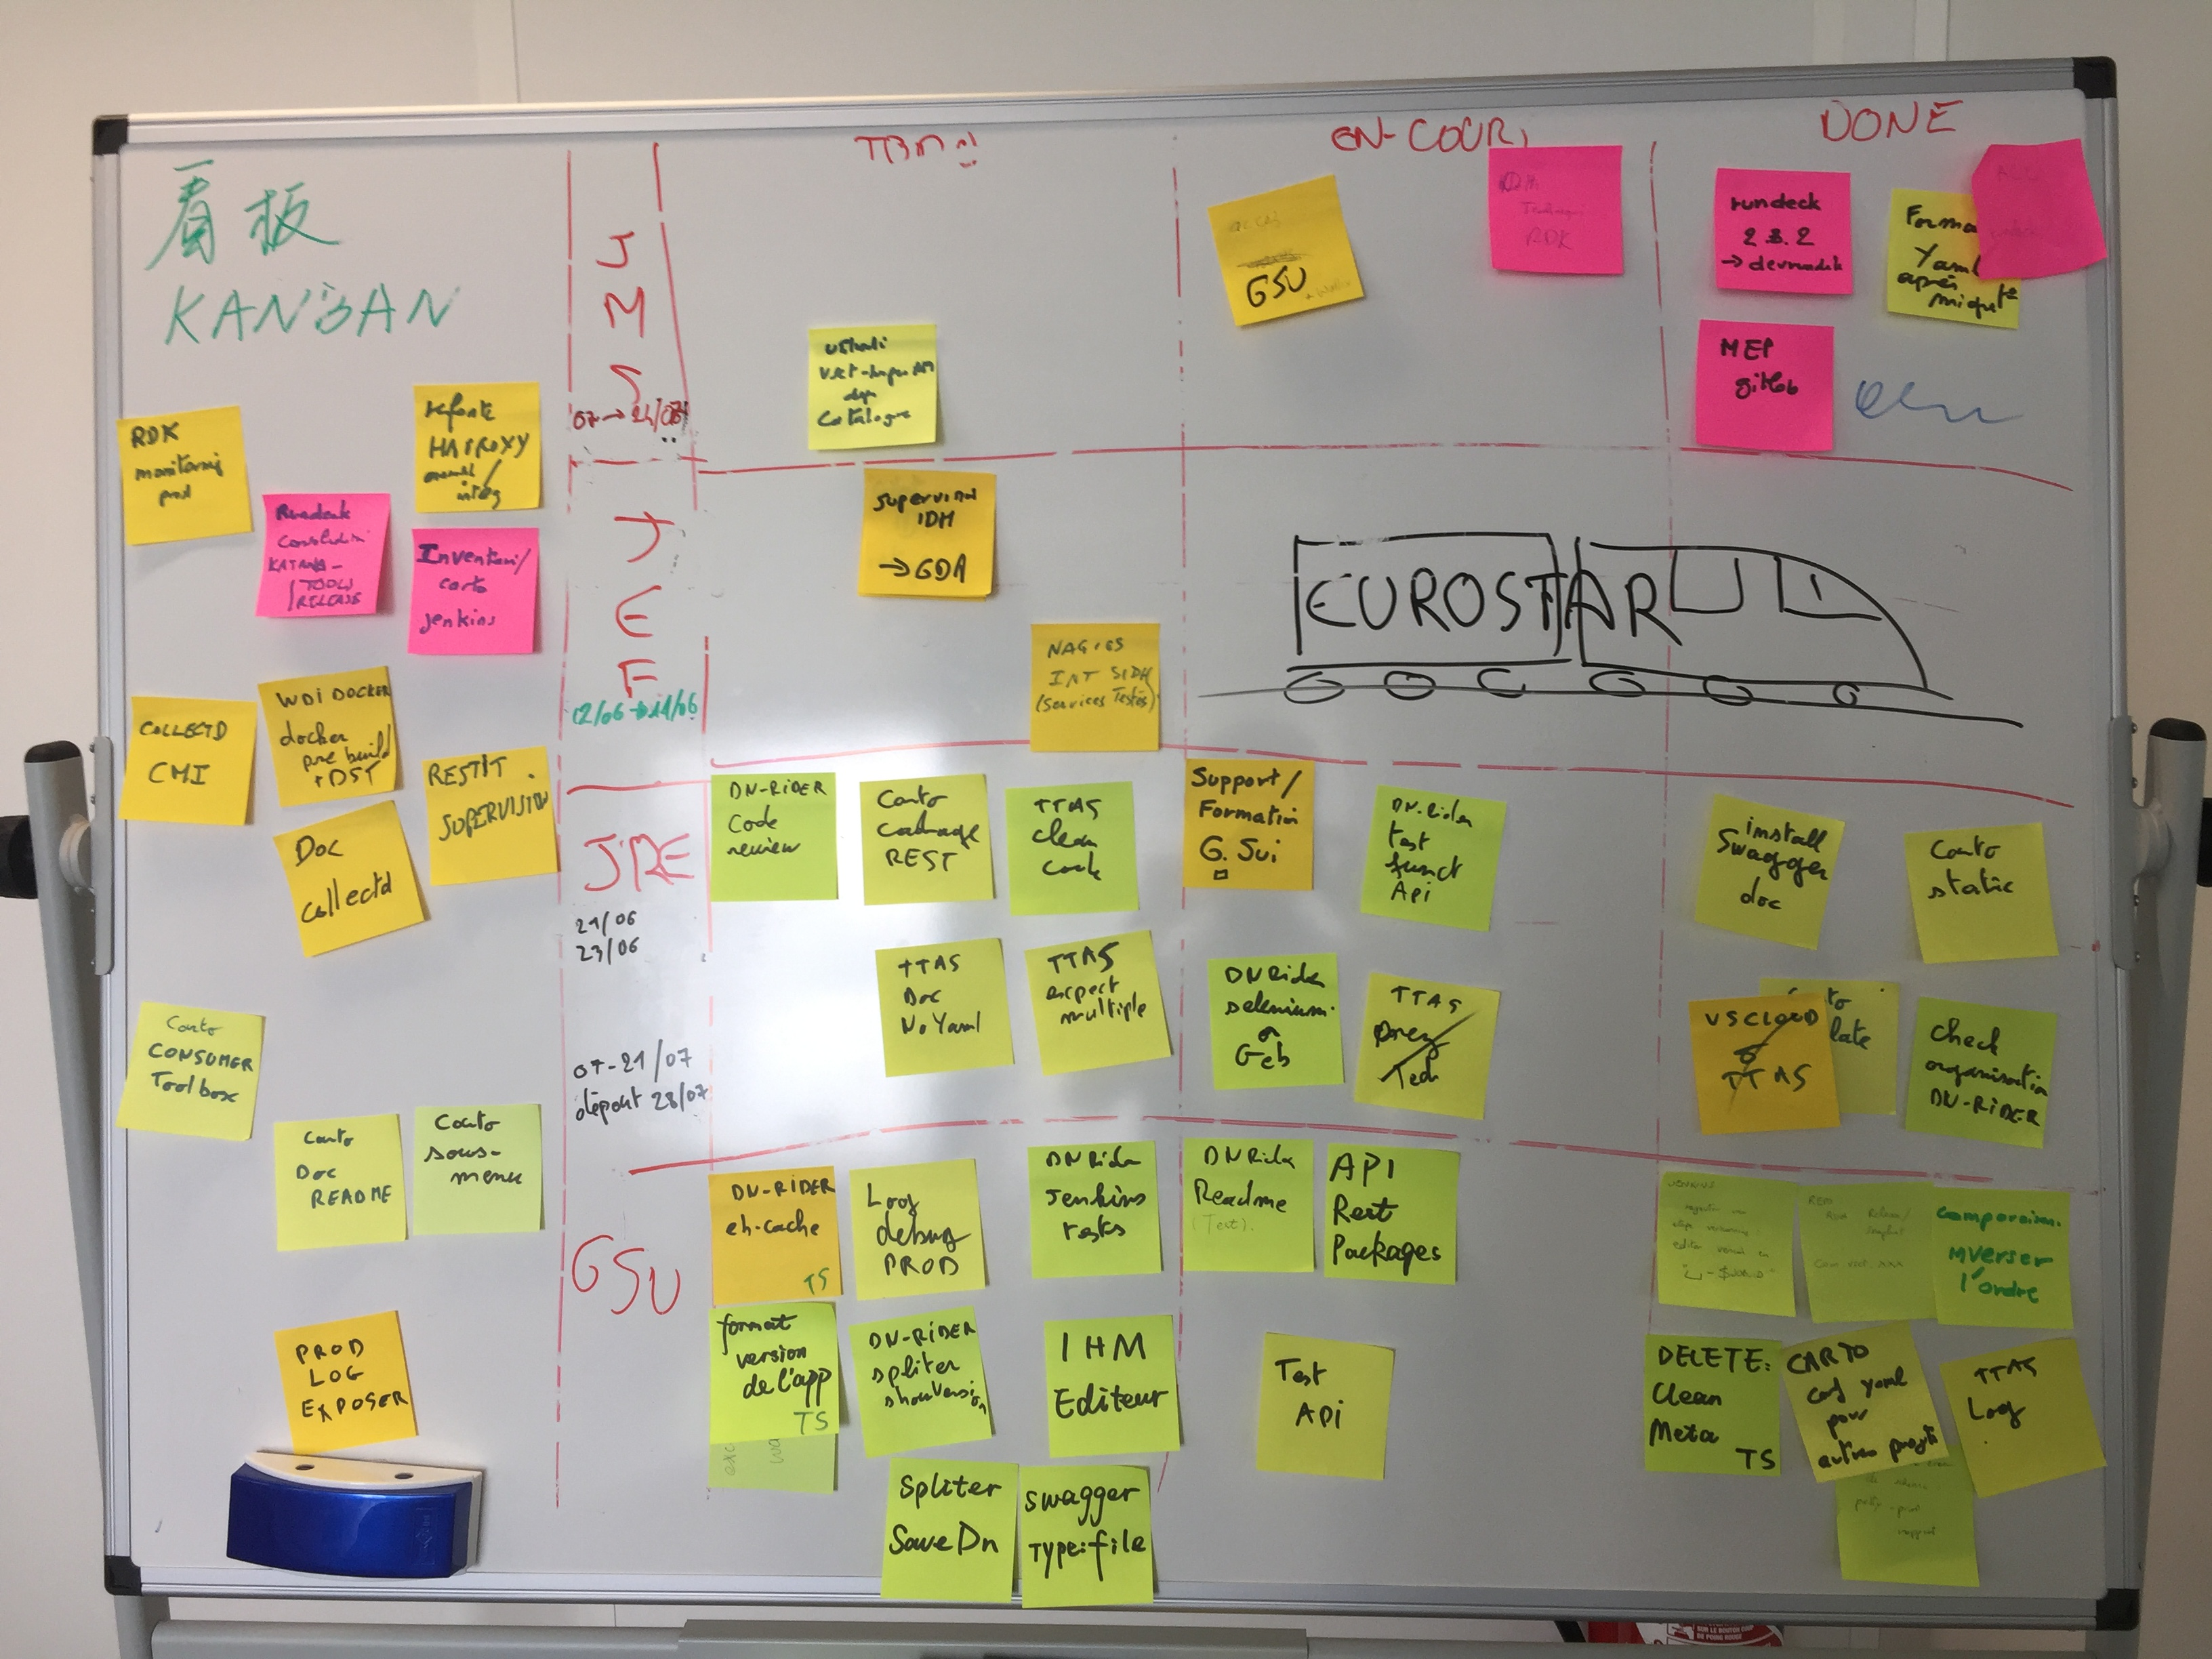
\includegraphics[width=0.8\textwidth]{kanban}
\caption{Kanban}
\end{figure}

\clearpage

\section{Application}
\paragraph{présentation: IHM, Api REST(swagger), Continus Delivery(git, test unitaire, pipeline->deploiement auto)}
\paragraph{arch}
\subparagraph{choix de techno: groovy, grails(référent compétent), bootstrap, jquery(justificatif)/backlog}
\subparagraph{archi appli: modèle MVC, lien vers Nexus}

\clearpage

\section{Etat fin de stage}
\paragraph{1 application opérationnelle sur serveur PROD}
\paragraph{démo au sein de l’équipe (FUTUR démo global)}
\paragraph{bilan objectif de l’appli}

\clearpage

\chapter{Conclusion}
\label{chap:Conclusion}

\section{Bilan personnel}
C'était ma première expérience de travailler dans une grande entreprise informatique.
Ce stage a été très enrichissant pour moi,
car il m’a permis de découvrir les aspects d'une entreprise informatique et expérimenter le processus de développement.

\section{Bilan technique}
Grâce à ce projet, j'ai pu avoir ma première expérience en tant que développeur full-stack.

J'ai pu appliquer les différents frameworks de côté serveur et de côté client (Grails 3, Bootstrap 4, jQuery, jQueryUI).
J'ai pu pratiquer les langages que je connaisais (HTML, CSS, JavaScript, Java)
et j'ai eu la chance d'utiliser les langages que je ne connais pas (Bash, SCSS, Groovy) et les normes récentes (ECMAScript 6).
J'ai pu expérimenter l'environnement open-source.

Au niveau de gestion des codes, j'ai pris une basique connaissance de git et les méthodes d'organisation des branches et des merge requestes.

J'ai pu participer au déploiement manuel de l'application et ensuite à la réalisation de l'intégration continue.
J'ai pu observer la façon de travailler des spécialistes et ensuite créé un petit bout de scripts comme ce qu'ils ont fait.

Ce qui est le plus important,
je me forme progressivement l'habitude de chercher des informations dans les documentations officielles des frameworks, des plugins et des langages,
je commence à comprendre comment chercher mes questions précises dans les moteurs de recherche comme "Google" et les communautés comme "Stack Overflow",
je me sens plus capable qu'avant de trouver les problèmes et les résoudre.

\section{Bilan organisation et académique}
J'ai eu la chance de travailler en autonomie et d'être aidé par une équipe.
Le contexte était contraignant au niveau de temps, cahier des charges et contrat,
j'ai eu la liberté d'organiser mon travail.
J'ai bénéficié l'organisation transverse de l'équipe et j'ai pu pratiquer la méthode agile du développement.

\chapter{Lexique}

\section{Lexique Général}

\paragraph{EPIC: }
\label{lexi:epic}
Établissement public à caractère industriel et commercial.

\paragraph{Nexus : }
\label{lexi:nexus}
Nexus est un entrepôt de binaires.

\paragraph{Apache Lucène :}
\label{lexi:lucene}
Apache Lucène est un moteur d'indexation textuel. Il est utilisé par Nexus.

\paragraph{Kanban : }
\label{lexi:kanban}
Kanban est une méthode de gestion des connaissances relatives au travail,
qui met l’accent sur une organisation de type Juste-à-temps en fournissant l'information ponctuellement aux membres de l'équipe afin de ne pas les surcharger.
Dans cette approche, le processus complet de l'analyse des tâches jusqu’à leur livraison au client est consultable par tous les participants,
chacun prenant ses tâches depuis une file d'attente.

\paragraph{Devops : }
\label{lexi:devops}
Le devops est un mouvement visant à l'alignement de l'ensemble des équipes du système d'information sur un objectif commun,
à commencer par les équipes de dev ou dev engineers chargés de faire évoluer le système d'information et les ops ou ops engineers responsables des infrastructures (exploitants, administrateurs système, réseau, bases de données,...).
Ce qui peut être résumé par : travailler ensemble pour produire de la valeur pour l'entreprise.

\paragraph{SCRUM : }
\label{lexi:scrum}
C’est une méthode « hyper procédurière » de conduite de projet agile.
« Hyper procédurière » car elle s’appuie sur un ensemble de rituels tels que le daily meeting, la démonstration, le sprint planning, etc.

\paragraph{Ajax : }
\label{lexi:ajax}
Ajax (Asynchronous JavaScript And Xml) est un ensemble de techniques de développement Web en utilisant de nombreuses technologies Web sur le côté client pour créer des applications Web asynchrones.

\section{Lexique de VSC Technologies}

\paragraph{Note de livraison : }
\label{lexi:delivery_note}
Une note de livraison est un fichier qui fait le lien entre la vue technique et la vue applicative.

\paragraph{Trigramme : }
\label{lexi:trigramme}
Un trigramme est l'identifiant d'une application.
Historiquement, cet identifiant se ramène à un code sur trois caractères.


\end{document}
